\documentclass[a4paper,twoside]{article}
%DIF LATEXDIFF DIFFERENCE FILE
%DIF DEL /home/resort/Documents/repos/AgenticPerformanceMonitor/paper/draft_v1/main.tex   Sat Nov 14 11:57:01 2026
%DIF ADD /home/resort/Documents/repos/AgenticPerformanceMonitor/paper-revised/main.tex    Sat Nov 14 12:25:02 2026
\usepackage{graphicx}
\usepackage{calc}
\usepackage{amssymb}
\usepackage{amstext}
\usepackage{amsmath}
\usepackage{amsthm}
\usepackage{multicol}
\usepackage{pslatex}
\usepackage{apalike}
\usepackage{algorithm2e}
\usepackage[bottom]{footmisc}
\usepackage[T1]{fontenc}
\usepackage[utf8]{inputenc}
\usepackage{url}
\usepackage{SCITEPRESS}
\pdfinfo{/Title (Agentic Dashboards: Numerical Validity, Answer Completeness, and with Adaptive Presentation) /Author () /Subject (Anonymous author-review manuscript draft) /Keywords (Analytical agents; evidence provenance; longitudinal dashboards)}
% BEGIN GENERATED: numbers
\newcommand{\EnumVisible}{24}
\newcommand{\EnumSelected}{24}
\newcommand{\EnumAccepted}{24}
\newcommand{\AVisible}{21}
\newcommand{\ASelected}{18}
\newcommand{\AAccepted}{22}
\newcommand{\BVisible}{15}
\newcommand{\BSelected}{14}
\newcommand{\BAccepted}{24}
\newcommand{\CVisible}{15}
\newcommand{\CSelected}{11}
\newcommand{\CAccepted}{21}
% END GENERATED: numbers
\newcommand{\draftassist}{\footnote{Writing assistance: OpenAI Codex \cite{openaiCodex}; see Section~\ref{sec:disclosure}.}}
%DIF PREAMBLE EXTENSION ADDED BY LATEXDIFF
%DIF UNDERLINE PREAMBLE %DIF PREAMBLE
\RequirePackage[normalem]{ulem} %DIF PREAMBLE
\RequirePackage{color}\definecolor{RED}{rgb}{1,0,0}\definecolor{BLUE}{rgb}{0,0,1} %DIF PREAMBLE
\providecommand{\DIFadd}[1]{{\protect\color{blue}\uwave{#1}}} %DIF PREAMBLE
\providecommand{\DIFdel}[1]{{\protect\color{red}\sout{#1}}}                      %DIF PREAMBLE
%DIF SAFE PREAMBLE %DIF PREAMBLE
\providecommand{\DIFaddbegin}{} %DIF PREAMBLE
\providecommand{\DIFaddend}{} %DIF PREAMBLE
\providecommand{\DIFdelbegin}{} %DIF PREAMBLE
\providecommand{\DIFdelend}{} %DIF PREAMBLE
\providecommand{\DIFmodbegin}{} %DIF PREAMBLE
\providecommand{\DIFmodend}{} %DIF PREAMBLE
%DIF FLOATSAFE PREAMBLE %DIF PREAMBLE
\providecommand{\DIFaddFL}[1]{\DIFadd{#1}} %DIF PREAMBLE
\providecommand{\DIFdelFL}[1]{\DIFdel{#1}} %DIF PREAMBLE
\providecommand{\DIFaddbeginFL}{} %DIF PREAMBLE
\providecommand{\DIFaddendFL}{} %DIF PREAMBLE
\providecommand{\DIFdelbeginFL}{} %DIF PREAMBLE
\providecommand{\DIFdelendFL}{} %DIF PREAMBLE
%DIF LISTINGS PREAMBLE %DIF PREAMBLE
\RequirePackage{listings} %DIF PREAMBLE
\RequirePackage{color} %DIF PREAMBLE
\lstdefinelanguage{DIFcode}{ %DIF PREAMBLE
%DIF DIFCODE_UNDERLINE %DIF PREAMBLE
  moredelim=[il][\color{red}\sout]{\%DIF\ <\ }, %DIF PREAMBLE
  moredelim=[il][\color{blue}\uwave]{\%DIF\ >\ } %DIF PREAMBLE
} %DIF PREAMBLE
\lstdefinestyle{DIFverbatimstyle}{ %DIF PREAMBLE
	language=DIFcode, %DIF PREAMBLE
	basicstyle=\ttfamily, %DIF PREAMBLE
	columns=fullflexible, %DIF PREAMBLE
	keepspaces=true %DIF PREAMBLE
} %DIF PREAMBLE
\lstnewenvironment{DIFverbatim}{\lstset{style=DIFverbatimstyle}}{} %DIF PREAMBLE
\lstnewenvironment{DIFverbatim*}{\lstset{style=DIFverbatimstyle,showspaces=true}}{} %DIF PREAMBLE
%DIF END PREAMBLE EXTENSION ADDED BY LATEXDIFF

\begin{document}
\title{Agentic Dashboards: Numerical Validity, Answer Completeness, and Adaptive Presentation}
\author{}
\keywords{Analytical Agents, Longitudinal Data, Evidence Provenance, Answer Completeness, Adaptive Dashboards.}
\abstract{A question such as "Has this student's activity changed, and how does it compare with their peers?" often requires a dashboard to bring several kinds of information together. We present an agentic dashboard system that organizes real educational activity and assessment records into views suited to different questions. A language model chooses predefined analyses and selects results. Deterministic tools calculate the quantities, validation links them to supporting records, and presentation templates arrange the selected information. The dashboards highlight personal change, compare peer groups and time periods, distinguish recorded zeros from unavailable observations, and present assessment histories. Users can switch among saved comparisons and inspect the evidence behind displayed values. We evaluate three selection interfaces using Qwen2.5-14B-Instruct on 24 development cases from two Open University course offerings. The interfaces produced \AVisible, \BVisible, and \CVisible\ complete visible answers, respectively, compared with \EnumVisible\ for a deterministic baseline. We also distinguish answers selected by the model from information added automatically by the dashboard software. The saved outputs reveal that correct, traceable values can still refer to the wrong period or leave part of a question unanswered. More explicit analytical labels did not improve the original completeness scores, and some equivalent answer forms still require human review. The contribution combines a working adaptive dashboard system, concrete interface examples, and a comparative evaluation showing how analysis selection, evidence checking, and presentation jointly shape the answers users receive.}
\onecolumn\maketitle\normalsize\setcounter{footnote}{0}\vfill


\section{\uppercase{Introduction}}
\label{sec:intro}
\noindent Dashboards can help people understand how their activity changes over time and how it compares with that of others. The most useful view, however, depends on the question. A student asking about recent progress needs a comparison with their own earlier activity. A student asking how they compare with others needs a suitable peer group. If recent observations are unavailable, the dashboard should explain the gap instead of suggesting a trend.
This paper develops an agentic dashboard tool around that idea. Using educational activity and assessment records, the tool presents views for personal change, peer comparisons, limited observations, and assessment history. Each view brings the relevant information into focus. For example, a reference selector lets the user explore saved comparisons, while an observation timeline distinguishes weeks with no recorded activity from periods when the student was not eligible to participate.

The system combines a language model with predefined analysis tools and presentation templates. The model chooses analyses and selects results to answer the question. The tools calculate the values, and the software checks their supporting records before assembling the dashboard. A separate presentation layer arranges the selected information into the different views. This division makes the displayed results traceable while allowing the content to vary across questions.
We examine three ways of providing analytical information to the model. These range from a compact interface to richer descriptions of data availability and comparison scope, followed by explicit labels identifying the measure, periods, and reference group. The same model and calculation tools are used throughout. A deterministic baseline selects the required analyses through predefined rules for the same question families.

The evaluation asks whether clearer analytical descriptions help the model produce more complete answers. It also distinguishes information selected by the model from context added automatically by the dashboard software. Inspecting the saved outputs shows where the system answers the question successfully and where it retrieves correct information but chooses an unsuitable comparison or leaves part of the question unanswered.
The contribution is a working dashboard system, a comparison of its selection interfaces, and concrete examples of its behavior. More explicit labels did not improve the original completeness scores. Some alternative answer forms still require human review. The interface examples illustrate practical adaptation, while the evaluation identifies limitations to address in further development.


\section{\uppercase{Related Work}}
\label{sec:related}
\noindent \DIFdelbegin \DIFdel{Adaptive dashboards connect research on language interfaces, visualization authoring, and analytical evaluation. }\DIFdelend NL4DV connects natural language queries to data attributes, analytical tasks, and Vega-Lite specifications \cite{nl4dv}. NL4DV-LLM extends this approach with conversational interaction and ambiguity handling \cite{sah2024}. 
\DIFdelbegin \DIFdel{These systems motivate translating a user's question into explicit analytical choices. For longitudinal data, those choices include the measure, time periods, and whether the comparison concerns personal history or peers.
}%DIFDELCMD < 

%DIFDELCMD < %%%
\DIFdel{Those choices must then become a useful display. }\DIFdelend LIDA combines data summarization, goal exploration, visualization code generation and evaluation, and infographic generation \cite{lida}. Data Formulator~2 supports iterative authoring through graphical and natural language inputs, generated data transformations, and branching histories \cite{dataformulator2}. Our system adopts a narrower division of work. The model selects predefined analyses and results, while calculation tools and presentation templates produce the dashboard. 
\DIFdelbegin \DIFdel{This supports different views while keeping calculations and presentation rules available for inspection.
}%DIFDELCMD < 

%DIFDELCMD < %%%
\DIFdel{Declarative visualization provides a design model for this separation. }\DIFdelend Vega-Lite expresses visual encodings and interactions through specifications that compile into graphical displays \cite{vegalite}. Draco represents visualization design knowledge through hard and soft constraints \cite{draco}. \DIFdelbegin \DIFdel{Our templates similarly control how selected information becomes a view. Personal timelines, peer comparisons, and observation summaries can therefore use different presentations while retaining consistent meanings for values, periods, and availability.
These design choices also shape the evaluation. }\DIFdelend InsightBench studies agents that formulate questions, perform analyses, and summarize insights using datasets containing planted patterns \cite{insightbench}. Here, the questions are supplied, and the observations come from real educational records. We examine whether the model selects enough information to answer each question. 
\DIFdelbegin \DIFdel{Holding the calculation and presentation machinery fixed helps identify failures in selection, including choosing an earlier period when the question concerns recent activity.
}%DIFDELCMD < 

%DIFDELCMD < %%%
\DIFdelend VisEval further distinguishes executable validity, satisfaction of chart and data requirements, and readability \cite{viseval}. Its acceptance of multiple valid charts is particularly relevant to assessing our dashboards. A requested value may appear in different supported answer forms, so checking one expected representation can miss a valid response. This motivates separate checks of numerical support and answer completeness. Some equivalent forms in our development comparison still require human adjudication.
W3C PROV-DM provides concepts for describing entities, activities, agents, and derivations \cite{prov}. This perspective motivates tracking the source results, model selections, automatically supplied context, and final presentation separately. 
\DIFdelbegin \DIFdel{Together, these research strands inform our development of a longitudinal dashboard system and a comparative study connecting what the model selects, what the software adds, and what the user can inspect.
}\DIFdelend 

\section{\uppercase{Data and Analytical Definitions}}
\label{sec:data}
\noindent \DIFdelbegin \DIFdel{To help operators interpret changes in activity, the dashboards need consistent definitions of time, participation, and available records. }\DIFdelend We use the Open University Learning Analytics Dataset (OULAD), which links course offerings, registrations, assessments, and virtual learning environment interactions \cite{oulad}. The creator deposited UCI archive is distributed under CC BY~4.0 \cite{ouladDataset}. Our audit counted 28,785 distinct people, 32,593 registrations\DIFdelbegin \DIFdel{in course offerings}\DIFdelend , 173,912 assessment records, and 10,655,280 interaction rows. \DIFdelbegin \DIFdel{People and registrations are counted separately because a person can register more than once. To avoid multiplying counts when combining sources, we }\DIFdelend \DIFaddbegin \DIFadd{We }\DIFaddend checked duplicate keys and many-to-one joins and aggregated interaction and assessment records before constructing weekly features.

\subsection{Development Population and Time}
We selected \DIFdelbegin \DIFdel{two offerings from different modules, }\DIFdelend AAA\_2013J and BBB\_2013B \DIFdelbegin \DIFdel{, to develop dashboards with sufficient history for comparisons. Selection followed lexical orderand required }\DIFdelend \DIFaddbegin \DIFadd{in lexical order, requiring }\DIFaddend 100 development people with eight fully eligible weeks and two dated non-examination assessments by day~83. The offerings contained 254 and 1,269 development registrations, representing 1,523 distinct people. \DIFdelbegin \DIFdel{These criteria selected usable record structures without targeting unusually high or low activity.
}%DIFDELCMD < 

%DIFDELCMD < %%%
\DIFdel{A hash of person identifiers }\DIFdelend \DIFaddbegin \DIFadd{A hash }\DIFaddend assigned approximately 70\% of people to development and reserved 8,583 people, keeping all registrations for each person together. \DIFdelbegin \DIFdel{A global structural audit preceded preparation. }\DIFdelend Reserved observations were not used for case selection, fitting, prompt development, or the present comparison\DIFdelbegin \DIFdel{, which remains a development study}\DIFdelend .

\DIFdelbegin \DIFdel{Each dashboard summarizes activity by person, offering, and week. Day~0 marks the offering's start, and week}\DIFdelend \DIFaddbegin \DIFadd{Week}\DIFaddend ~$w$ covers days $7w$ through $7w+6$ \DIFaddbegin \DIFadd{from the offering's start}\DIFaddend . Only calendar weeks ending by the \DIFdelbegin \DIFdel{analytical }\DIFdelend cutoff are included. \DIFdelbegin \DIFdel{Within a week, eligibility }\DIFdelend \DIFaddbegin \DIFadd{Eligibility }\DIFaddend starts at registration and ends before the withdrawal day. Future withdrawal is masked, and unknown registration leaves eligibility unknown. These rules \DIFdelbegin \DIFdel{help distinguish gaps in participation from recorded inactivity. They }\DIFdelend reconstruct availability retrospectively and have not been validated as a real-time feed.

\subsection{Recorded Measures and Availability}
\DIFdelbegin \DIFdel{To account for differences in eligible time, we express recorded clicks as a daily rate. }\DIFdelend For person $i$ in week $w$, \DIFdelbegin \DIFdel{let $d_{iw}$ denote administratively eligible days and $c_{iw}$ the recorded clicks on those days . The rate is
}\begin{displaymath}
\DIFdel{x_{iw}=c_{iw}/d_{iw},\qquad d_{iw}>0.
%DIFDELCMD < \label{eq:rate}%%%
}\end{displaymath}%DIFAUXCMD
\DIFdel{The dashboard shows this rate as unavailable when eligibility is unknown or there are }\DIFdelend \DIFaddbegin \DIFadd{recorded clicks per eligible day are $x_{iw}=c_{iw}/d_{iw}$ when eligible days $d_{iw}>0$. Unknown eligibility or }\DIFaddend no eligible days \DIFdelbegin \DIFdel{. An }\DIFdelend \DIFaddbegin \DIFadd{makes the rate unavailable; an }\DIFaddend eligible week without recorded clicks receives zero. \DIFdelbegin \DIFdel{This distinction helps operators read gaps correctly, although logging }\DIFdelend \DIFaddbegin \DIFadd{Logging }\DIFaddend completeness remains unknown. \DIFdelbegin \DIFdel{Absent clicks establish neither logging failure nor lack of effort, and click }\DIFdelend \DIFaddbegin \DIFadd{Click }\DIFaddend counts do not measure ability, study time, or learning.

Other weekly measures \DIFdelbegin \DIFdel{provide complementary views of the records. These include }\DIFdelend \DIFaddbegin \DIFadd{are }\DIFaddend days with positive activity, distinct resources, non-banked submissions, and scheduled assessments without a recorded submission. Submissions count in their recorded week \DIFdelbegin \DIFdel{, }\DIFdelend within eligibility and the cutoff. The scheduled measure counts dated non-examination assessments due during \DIFdelbegin \DIFdel{an eligible part of the week }\DIFdelend \DIFaddbegin \DIFadd{eligibility }\DIFaddend without a non-banked submission by that week's end. \DIFdelbegin \DIFdel{It describes recorded opportunities, since unknown }\DIFdelend \DIFaddbegin \DIFadd{Unknown }\DIFaddend exemptions prevent interpreting every missing submission as an unmet obligation. Later submissions do not rewrite earlier status snapshots.

\DIFdelbegin \DIFdel{To keep historical views consistent with their cutoff, agent inputs }\DIFdelend \DIFaddbegin \DIFadd{Inputs }\DIFaddend exclude future activity, final results, and future withdrawal. \DIFdelbegin \DIFdel{Assessment scores }\DIFdelend \DIFaddbegin \DIFadd{Scores }\DIFaddend are withheld because submission dates do not establish \DIFdelbegin \DIFdel{when grades became available}\DIFdelend \DIFaddbegin \DIFadd{grade availability}\DIFaddend . Banked assessments \DIFdelbegin \DIFdel{transferred from earlier offerings are excluded from prospective counts }\DIFdelend \DIFaddbegin \DIFadd{are excluded }\DIFaddend because approval timing is unknown. \DIFdelbegin \DIFdel{Grade unavailability therefore reflects missing timing information, rather than insufficient sample size. All conditions use these rules.
}%DIFDELCMD < 

%DIFDELCMD < %%%
\DIFdel{Repeated source rows remain a measurement limitation. }\DIFdelend The primary analysis \DIFdelbegin \DIFdel{sums them, while the audit identified }\DIFdelend \DIFaddbegin \DIFadd{preserves repeated source rows: the audit found }\DIFaddend 787,170 exact duplicate excess rows and 2,195,960 excess rows under a candidate \DIFdelbegin \DIFdel{'}\DIFdelend person-offering-site-day \DIFdelbegin \DIFdel{' }\DIFdelend key. That key is not assumed to identify unique events. \DIFdelbegin \DIFdel{An earlier, limited sensitivity check removed exact duplicates, but it does not establish robustness across the present cases.
The interpretation of repeated rows still requires review.
}\DIFdelend \DIFaddbegin \DIFadd{Section~\ref{sec:sensitivity} reports a post hoc exact-row sensitivity for the current cases.
}\DIFaddend 

\subsection{Personal and Peer Comparisons}
\DIFdelbegin \DIFdel{The dashboard uses consistent summaries to connect personal progress with peer comparisons. }\DIFdelend Let $O_i(W)$ contain eligible weeks with recorded values \DIFdelbegin \DIFdel{for a feature }\DIFdelend in period $W$. The person's mean \DIFdelbegin \DIFdel{, unavailable when this set is empty, is
}\begin{displaymath}
\DIFdel{m_i(W)=\frac{1}{|O_i(W)|}\sum_{w\in O_i(W)}x_{iw}.
%DIFDELCMD < \label{eq:person}%%%
}\end{displaymath}%DIFAUXCMD
\DIFdelend \DIFaddbegin \DIFadd{is
}\begin{equation}
\DIFadd{m_i(W)=\frac{1}{|O_i(W)|}\sum_{w\in O_i(W)}x_{iw},
}\end{equation}
\DIFadd{unavailable when $O_i(W)$ is empty. }\DIFaddend Weeks receive equal weight, including partial weeks after calculating \DIFdelbegin \DIFdel{their daily rates. This differs from dividing total clicks by total }\DIFdelend \DIFaddbegin \DIFadd{daily rates; this differs from pooling clicks and }\DIFaddend eligible days. Personal change $\Delta_i=m_i(W_r)-m_i(W_b)$ requires \DIFdelbegin \DIFdel{at least }\DIFdelend two observed weeks in \DIFdelbegin \DIFdel{both the recent and earlier periods}\DIFdelend \DIFaddbegin \DIFadd{each period}\DIFaddend .

For reference group $g$ \DIFdelbegin \DIFdel{and }\DIFdelend \DIFaddbegin \DIFadd{in }\DIFaddend period $W_g$, \DIFdelbegin \DIFdel{let $P_g$ contain eligible }\DIFdelend peers with at least one nonmissing week \DIFdelbegin \DIFdel{. The peer mean and the person's difference from it are
}\begin{align*}
\DIFdel{\mu_g(W_g)}&\DIFdel{=\frac{1}{|P_g|}\sum_{j\in P_g}m_j(W_g),}\\
\DIFdel{D_{i,g}}&\DIFdel{=m_i(W_r)-\mu_g(W_g).
}\end{align*}%DIFAUXCMD
\DIFdel{Each person receives equal weight}\DIFdelend \DIFaddbegin \DIFadd{form $P_g$. Their equally weighted mean is $\mu_g(W_g)=|P_g|^{-1}\sum_{j\in P_g}m_j(W_g)$, and the focal difference is $D_{i,g}=m_i(W_r)-\mu_g(W_g)$}\DIFaddend . Comparisons require 20 peers and two \DIFdelbegin \DIFdel{observed weeksfor the person being assessed. Means may }\DIFdelend \DIFaddbegin \DIFadd{focal weeks; individual means can }\DIFaddend remain available below these \DIFdelbegin \DIFdel{thresholds. These prototype rules are not validated educational decision criteria}\DIFdelend \DIFaddbegin \DIFadd{prototype thresholds}\DIFaddend .

\DIFdelbegin \DIFdel{Operators can examine }\DIFdelend \DIFaddbegin \DIFadd{The }\DIFaddend three reference groups \DIFdelbegin \DIFdel{using these shared definitions. They }\DIFdelend include other development students in the \DIFdelbegin \DIFdel{same offering, students additionally }\DIFdelend \DIFaddbegin \DIFadd{offering, those }\DIFaddend sharing first-attempt or repeat-attempt status, and \DIFdelbegin \DIFdel{same-offering peers observed }\DIFdelend \DIFaddbegin \DIFadd{offering peers }\DIFaddend in the earlier period. \DIFdelbegin \DIFdel{The person being assessed and all other designated }\DIFdelend \DIFaddbegin \DIFadd{All }\DIFaddend task participants are excluded \DIFdelbegin \DIFdel{from peer groups across their registrations. These alternatives make the choice of comparison visible. }\DIFdelend \DIFaddbegin \DIFadd{across registrations. }\DIFaddend Earlier-period comparisons \DIFdelbegin \DIFdel{can differ in membership, observed history, and actual exposure, so }\DIFdelend \DIFaddbegin \DIFadd{change time and potentially membership; }\DIFaddend they are not necessarily fairer or causally adjusted. Weekly \DIFdelbegin \DIFdel{peer }\DIFdelend trajectories always use \DIFdelbegin \DIFdel{eligible peersfrom the same week, even when an accompanying summary uses an earlier reference period}\DIFdelend \DIFaddbegin \DIFadd{same-week peers}\DIFaddend .

\DIFdelbegin \DIFdel{To show uncertainty around peer means, we }\DIFdelend \DIFaddbegin \DIFadd{We }\DIFaddend draw 500 seeded bootstrap samples of people\DIFdelbegin \DIFdel{with replacement, retain each person's period mean}\DIFdelend \DIFaddbegin \DIFadd{, retaining their period means}\DIFaddend , and use the 2.5th and 97.5th percentiles \cite{efron}. Weekly bands repeat this \DIFdelbegin \DIFdel{procedure separately for each weekand describe uncertainty at each point, rather than across the whole trajectory}\DIFdelend \DIFaddbegin \DIFadd{separately by week}\DIFaddend . No interval is shown with fewer than two peers. \DIFdelbegin \DIFdel{These intervals describe }\DIFdelend \DIFaddbegin \DIFadd{Intervals concern }\DIFaddend peer means only\DIFdelbegin \DIFdel{. They do not predict individual activity or quantify uncertainty in }\DIFdelend \DIFaddbegin \DIFadd{, not individual predictions, }\DIFaddend personal change, \DIFdelbegin \DIFdel{$D_{i,g}$}\DIFdelend \DIFaddbegin \DIFadd{focal differences}\DIFaddend , or differences between \DIFdelbegin \DIFdel{reference choices. Fixed seeds make the calculations reproducible without establishing generalization beyond the selected offerings. The dashboards use these descriptive calculations. A separate exploratory mixed-model analysis is not a validated detector and supplies no dashboard claims}\DIFdelend \DIFaddbegin \DIFadd{references}\DIFaddend .

\section{\uppercase{From Questions to Dashboards}}
\label{sec:system}
\noindent \DIFdelbegin \DIFdel{Our approach connects flexible analysis selection with checked calculations and reusable views (Figure~1). }\DIFdelend The model receives the person, offering, cutoff, periods, task family, question, and shared feature/reference definitions. Structured requests let it run analytical batches, inspect compact results, and request more information or finish. Evaluation-only requirements remain hidden, and generated analysis code is not executed.

\DIFdelbegin %DIFDELCMD < \begin{figure*}[!t]
%DIFDELCMD < \centering
%DIFDELCMD < \includegraphics[width=\textwidth]{figures/architecture.pdf}
%DIFDELCMD < %%%
%DIFDELCMD < \caption{%
{%DIFAUXCMD
\DIFdelFL{From analytical choices to inspectable dashboards. The agent selects analyses and answer content, while deterministic tools calculate values. Evidence checks can reject an answer or allow one repair. The compiler adds labeled structure and context without filling in missing comparison claims. A later presentation layer organizes saved accepted outputs, and its reference selector works without another model call. Numerical correctness and answer completeness are checked separately.}}
%DIFAUXCMD
%DIFDELCMD < \label{fig:architecture}
%DIFDELCMD < \end{figure*}
%DIFDELCMD < 

%DIFDELCMD < %%%
\DIFdelend \subsection{Evidence and Answer Validation}
Evidence records \DIFdelbegin \DIFdel{connect each result to its feature}\DIFdelend \DIFaddbegin \DIFadd{retain features}\DIFaddend , units, periods, counts, estimates, support, observation and assessment states, \DIFdelbegin \DIFdel{and uncertainty. They also retain source and configuration hashes, random seeds, and execution details}\DIFdelend \DIFaddbegin \DIFadd{uncertainty, and source/configuration hashes}\DIFaddend . The model receives summaries rather than raw rows\DIFdelbegin \DIFdel{, while full evidence remains available for inspection. }%DIFDELCMD < 

%DIFDELCMD < %%%
\DIFdelend \DIFaddbegin \DIFadd{. }\DIFaddend Each peer comparison is identified by \DIFdelbegin \begin{displaymath}
\DIFdel{I_{\mathrm{peer}}=(i,o,t,f,W_f,g,W_g),
}\end{displaymath}%DIFAUXCMD
\DIFdel{where $i$ is the person, $o$ the offering, $t$ the cutoff, $f$ the feature, $W_f$ the person's period, $g$ the }\DIFdelend \DIFaddbegin \DIFadd{$I_{\mathrm{peer}}=(i,o,t,f,W_f,g,W_g)$: person, offering, cutoff, feature, focal period, }\DIFaddend reference group, and \DIFdelbegin \DIFdel{$W_g$ its }\DIFdelend \DIFaddbegin \DIFadd{reference }\DIFaddend period. A personal comparison instead uses \DIFdelbegin \begin{displaymath}
\DIFdel{I_{\mathrm{personal}}=(i,o,t,f,W_b,W_r),
}\end{displaymath}%DIFAUXCMD
\DIFdel{where $W_b$ and $W_r$ are the earlier and recent periods. Readable identifiers }\DIFdelend \DIFaddbegin \DIFadd{$I_{\mathrm{personal}}=(i,o,t,f,W_b,W_r)$, omitting peer meaning. Identifiers }\DIFaddend are generated only for returned evidence, without \DIFdelbegin \DIFdel{using }\DIFdelend hidden expected answers.

Unknown, ambiguous, or altered identifiers are rejected without substitution\DIFdelbegin \DIFdel{or additional analysis}\DIFdelend . Repeated personal summaries are equivalent only when their person, feature, units, cutoff, periods, means, counts, change, and support match exactly. \DIFdelbegin \DIFdel{The system consistently selects one returned identifier and preserves the alternatives without creating a peer comparison}\DIFdelend \DIFaddbegin \DIFadd{One returned identifier is selected consistently and its alternatives preserved}\DIFaddend .

Validation \DIFdelbegin \DIFdel{checks results against the trusted development data, including }\DIFdelend \DIFaddbegin \DIFadd{independently checks }\DIFaddend summaries, trajectories, counts, intervals, units, groups, periods, and eligibility \DIFaddbegin \DIFadd{against trusted development data}\DIFaddend . Changing values and recomputing their hash cannot bypass these checks. \DIFdelbegin \DIFdel{Displayed numbers must refer to validated fields, and unsupported scopes or identifiers fail even in correctly formatted responses. These checks establish consistency with the implementation, while scientific adequacy and answer completenessrequire separate assessment}\DIFdelend \DIFaddbegin \DIFadd{Numerical consistency does not establish answer completeness}\DIFaddend .

\subsection{Building and Tracing Answers}
\DIFdelbegin \DIFdel{The dashboard supports peer comparisons, personal change, assessment status, observation status, and measurement limitations. Selected }\DIFdelend \DIFaddbegin \DIFadd{Selected peer }\DIFaddend comparisons become claims and panels\DIFdelbegin \DIFdel{, while }\DIFdelend \DIFaddbegin \DIFadd{; }\DIFaddend personal results become claims and trajectories. Support rules determine whether \DIFdelbegin \DIFdel{the }\DIFdelend wording describes a result or explains insufficient observations. Unknown grades remain unavailable measurements. \DIFdelbegin %DIFDELCMD < 

%DIFDELCMD < %%%
\DIFdelend The compiler adds required timelines, observation and assessment context, and qualifications without filling in missing comparison or personal claims. These additions can still answer a requested item, such as grade availability. Provenance \DIFdelbegin \DIFdel{therefore }\DIFdelend records model selections, identifier resolution, metadata, and compiler additions separately. All numerical calculation and insertion are deterministic.
\DIFdelbegin \DIFdel{Model selection determines which content appears.
}\DIFdelend 

\subsection{Adaptive Presentation of Saved Answers}
The publication views \DIFdelbegin \DIFdel{were created }\DIFdelend \DIFaddbegin \DIFadd{reorganize saved content }\DIFaddend after the experiment\DIFdelbegin \DIFdel{by reorganizing saved content}\DIFdelend . They introduce no evidence, \DIFdelbegin \DIFdel{changed periods, }\DIFdelend corrected omissions, or revised scores. Layout follows content rather than case identifiers. Equivalent personal duplicates may be combined with \DIFdelbegin \DIFdel{their }\DIFdelend original multiplicity recorded\DIFdelbegin \DIFdel{, while }\DIFdelend \DIFaddbegin \DIFadd{; }\DIFaddend distinct peer claims remain available\DIFdelbegin \DIFdel{in expanded views}\DIFdelend . Evaluation uses \DIFdelbegin \DIFdel{the }\DIFdelend complete original dashboards.

Figure~\ref{fig:adaptation} shows \DIFdelbegin \DIFdel{how presentation changes with the available information. Personal views emphasize trajectories and selected peer comparisons. Observation viewsdistinguish recorded zeros, ineligibility, and unavailable quantities, using timelines and grade context already supplied by the original compiler. Assessment views emphasize submissions per observed week and dated records. Every view includes expandable evidenceand information about sources and methods. }%DIFDELCMD < 

%DIFDELCMD < \begin{figure*}[!t]
%DIFDELCMD < \centering
%DIFDELCMD < 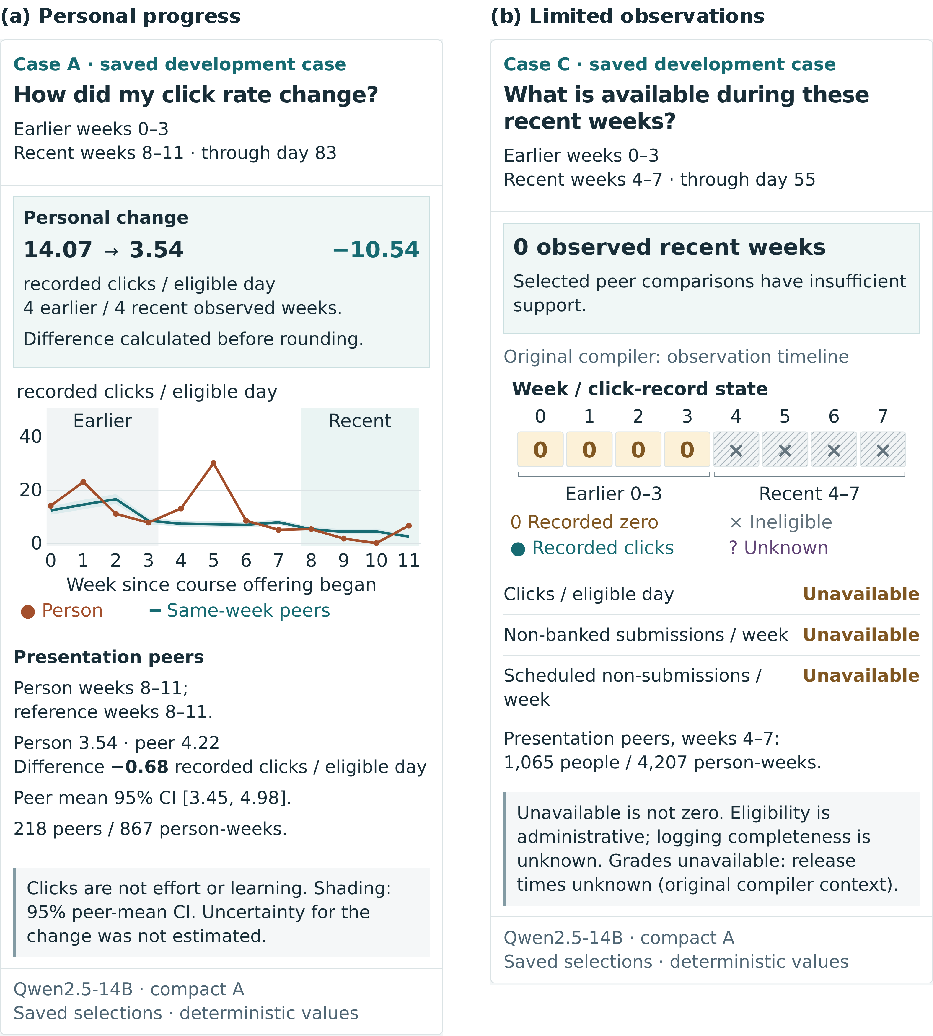
\includegraphics[width=\textwidth]{figures/adaptation.pdf}
%DIFDELCMD < %%%
%DIFDELCMD < \caption{%
{%DIFAUXCMD
\DIFdelFL{Adapted views of saved answers from compact condition A. (a) Case 01 shows selected personal change and recent peer context. Change uses unrounded means. Shading represents pointwise 95\% bootstrap intervals for peer means, not personal change. (b) Case 09 separates recorded zeros from ineligibility and unavailable recent values. It was accepted after one historical repair. Its original compiler supplied the observation timeline and grade context. Anonymous display aliases differ from condition labels. These examples demonstrate presentation behavior without establishing improved accuracy or usability.}}
%DIFAUXCMD
%DIFDELCMD < \label{fig:adaptation}
%DIFDELCMD < \end{figure*}
%DIFDELCMD < 

%DIFDELCMD < %%%
\DIFdel{In }\DIFdelend \DIFaddbegin \DIFadd{personal and limited-observation views. All views retain expandable evidence, zero/unavailable distinctions, and intervals for peer means only. }\DIFaddend Figure~\ref{fig:reference} \DIFdelbegin \DIFdel{, the selector switches between two comparisonsalready chosen by the same agent. Values}\DIFdelend \DIFaddbegin \DIFadd{switches between saved model-selected comparisons: values}\DIFaddend , counts, labels, charts, and evidence links update together \DIFdelbegin \DIFdel{while the person's measurement stays fixed. The interaction reads saved results }\DIFdelend without recalculation or new analysis.
\DIFdelbegin \DIFdel{All views preserve the distinction between zero and unavailable values, and intervals describe peer means rather than uncertainty in the comparison difference.
}\DIFdelend \DIFaddbegin 

\begin{figure*}[!t]
\centering
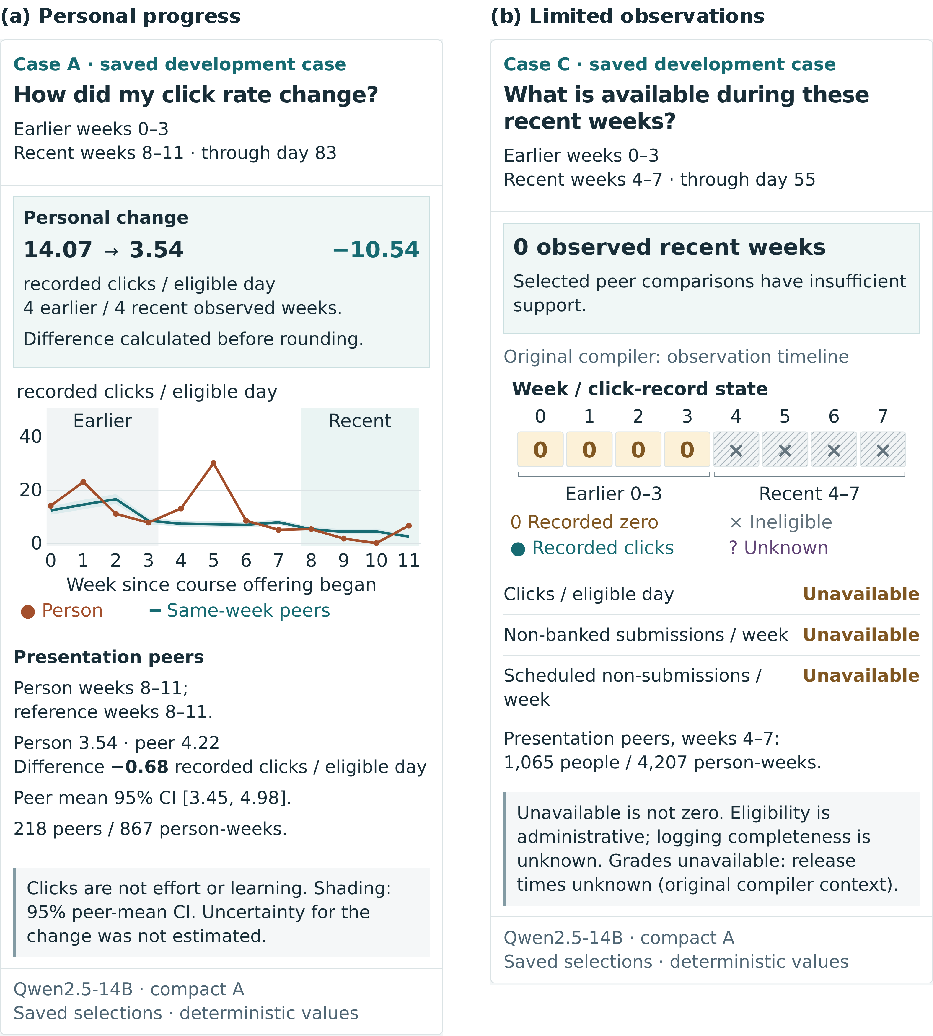
\includegraphics[width=0.9\textwidth]{figures/adaptation.pdf}
\caption{\DIFaddFL{Saved compact-A answers. (a) Case 01: personal change and recent peer context; change uses unrounded means. Shading gives pointwise 95\% bootstrap intervals for peer means, not personal change. (b) Case 09: zeros, ineligibility, and unavailable recent values. Its observation timeline and grade context were compiler supplied; acceptance followed one repair. These examples do not establish educational or usability improvements.}}
\label{fig:adaptation}
\end{figure*}
\DIFaddend 

\section{\uppercase{Experiment}}
\label{sec:experiment}
\noindent Four conditions answer identical questions about 24 additional development participants, \DIFdelbegin \DIFdel{with four cases }\DIFdelend \DIFaddbegin \DIFadd{four }\DIFaddend per question family. Earlier development established the backend, \DIFdelbegin \DIFdel{agent }\DIFdelend policy, compiler, and evaluator\DIFdelbegin \DIFdel{. Its }\DIFdelend \DIFaddbegin \DIFadd{; its }\DIFaddend participants are excluded \DIFdelbegin \DIFdel{from the new cases, }\DIFdelend and its results are not pooled \DIFdelbegin \DIFdel{with this comparison}\DIFdelend \DIFaddbegin \DIFadd{here}\DIFaddend .

\subsection{Cases and Shared Information}
The six \DIFdelbegin \DIFdel{question }\DIFdelend families address personal change alongside peers, \DIFdelbegin \DIFdel{comparisons between }\DIFdelend named reference groups, observation availability, separate \DIFdelbegin \DIFdel{limits on personaland recent peer comparisons, assessment submission and scheduled non-submission }\DIFdelend \DIFaddbegin \DIFadd{personal/peer insufficiency, assessment }\DIFaddend means with grade context, and alternative \DIFdelbegin \DIFdel{comparison periods. Reference questions do not automatically require personal change or a revised conclusion.
}%DIFDELCMD < 

%DIFDELCMD < %%%
\DIFdel{The fixed profiles }\DIFdelend \DIFaddbegin \DIFadd{periods. Profiles }\DIFaddend compare weeks 0--3 with 8--11 at day~83, 0--3 with 4--7 at day~55, 0--1 with 2--3 at day~27, 0--3 with 10--11 at day~83, and 2--5 with 6--9 at day~69. \DIFdelbegin \DIFdel{Each question specifies its }\DIFdelend \DIFaddbegin \DIFadd{Questions specify }\DIFaddend measure, periods, and cutoff.
\DIFaddbegin 

\DIFaddend Selection uses administrative eligibility and previous attempt status where relevant\DIFdelbegin \DIFdel{. Cases testing insufficient observations }\DIFdelend \DIFaddbegin \DIFadd{, never activity magnitudes or model outcomes. Insufficiency cases }\DIFaddend require fewer than two recent eligible weeks and at least one earlier \DIFdelbegin \DIFdel{eligible week. Selection does not target model failures or extreme activity.
}%DIFDELCMD < 

%DIFDELCMD < %%%
\DIFdel{For each case, we select }\DIFdelend \DIFaddbegin \DIFadd{week. We choose }\DIFaddend the unused eligible person with the smallest SHA256(seed, case, person), using seed \texttt{stage6-structural-v1-20260918}. All 57 previous and 24 new task participants are excluded from \DIFdelbegin \DIFdel{the shared peer pool }\DIFdelend \DIFaddbegin \DIFadd{peer pools }\DIFaddend across registrations. \DIFdelbegin \DIFdel{Cases use real observations. Separate calculations over source rows }\DIFdelend \DIFaddbegin \DIFadd{Separate row-based calculations }\DIFaddend checked 52 fact records\DIFdelbegin \DIFdel{, providing an independent computational check rather than }\DIFdelend \DIFaddbegin \DIFadd{; this is computational checking, not }\DIFaddend human review.

All conditions share questions, family labels, definitions, \DIFdelbegin \DIFdel{references, periods, }\DIFdelend and interpretation rules. \DIFdelbegin \DIFdel{Hidden facts support only scoring and later diagnosis. }\DIFdelend Tasks, prompts, code, \DIFdelbegin \DIFdel{schemas, }\DIFdelend sources, settings, scoring, and \DIFdelbegin \DIFdel{execution order were fixed before inference. There was no }\DIFdelend \DIFaddbegin \DIFadd{order were frozen before inference, without }\DIFaddend subsequent tuning or \DIFdelbegin \DIFdel{repetition of runs }\DIFdelend \DIFaddbegin \DIFadd{reruns }\DIFaddend to obtain success. \DIFaddbegin \DIFadd{Hidden facts support only scoring and diagnosis.
}\DIFaddend 

\subsection{Conditions and Ablation}
\textbf{Enumeration} follows rules for \DIFdelbegin \DIFdel{the public question families and available references . It requests applicable reference comparisons and any required assessment measures. It uses the same }\DIFdelend \DIFaddbegin \DIFadd{public families and references using the shared }\DIFaddend backend, validator, renderer, and \DIFdelbegin \DIFdel{limit of six tool calls. Its access to family labels makes }\DIFdelend \DIFaddbegin \DIFadd{six-call limit. Family labels make }\DIFaddend it a strong baseline for \DIFdelbegin \DIFdel{these }\DIFdelend defined tasks, without implying general language understanding.

\textbf{A, compact} selects answer types and returned identifiers, with \DIFdelbegin \DIFdel{the model specifying }\DIFdelend \DIFaddbegin \DIFadd{model-specified }\DIFaddend support and conclusion scope.
\DIFdelbegin \DIFdel{The existing compiler constructs the dashboard.
}%DIFDELCMD < 

%DIFDELCMD < %%%
\DIFdelend \textbf{B, derived metadata} retains these selections but \DIFdelbegin \DIFdel{determines }\DIFdelend \DIFaddbegin \DIFadd{derives }\DIFaddend support and scope\DIFdelbegin \DIFdel{automatically}\DIFdelend , uses a neutral heading, and supplies a catalogue of returned answers. \DIFdelbegin \DIFdel{Comparing B with A therefore tests this }\DIFdelend \DIFaddbegin \DIFadd{B--A tests that }\DIFaddend combined interface change.
\DIFdelbegin %DIFDELCMD < 

%DIFDELCMD < %%%
\DIFdelend \textbf{C, explicit binding} selects exact analytical identifiers \DIFdelbegin \DIFdel{while retaining }\DIFdelend \DIFaddbegin \DIFadd{with }\DIFaddend B's \DIFdelbegin \DIFdel{automatic }\DIFdelend metadata and identical catalogue. \DIFdelbegin \DIFdel{Comparing C with B tests how answers are identified while keeping available information equivalent. Comparing C with A }\DIFdelend \DIFaddbegin \DIFadd{C--B tests selection representation; C--A }\DIFaddend tests the full intervention. \DIFdelbegin \DIFdel{None receives hidden scoring requirements or automatically supplied }\DIFdelend \DIFaddbegin \DIFadd{No interface supplies hidden requirements or }\DIFaddend missing comparisons.
\DIFdelbegin \DIFdel{An agent can still select a valid result that does not answer the question.
}\DIFdelend 

\subsection{Model, Budgets and \DIFdelbegin \DIFdel{Ordering}\DIFdelend \DIFaddbegin \DIFadd{Outcomes}\DIFaddend }
Agents use Qwen2.5-14B-Instruct \cite{qwenReport,qwenCheckpoint}, revision \texttt{cf98f3b3bbb457ad9e2bb}\allowbreak\texttt{7baf9a0125b6b88caa8}\DIFdelbegin \DIFdel{. We use }\DIFdelend \DIFaddbegin \DIFadd{, }\DIFaddend Transformers 4.55.2, \DIFdelbegin \DIFdel{the checkpoint's tokenizer and chat template, Torch 2.8.0+cu128, CUDA~12.8, }\DIFdelend \DIFaddbegin \DIFadd{greedy decoding, and }\DIFaddend BF16 \DIFdelbegin \DIFdel{, and scaled dot-product attention. Parameters, inputs, and outputs remained }\DIFdelend on one RTX~6000 Ada GPU without quantization or \DIFdelbegin \DIFdel{CPU offload. CUDA profiling confirmed GPU execution.
}%DIFDELCMD < 

%DIFDELCMD < %%%
\DIFdel{Greedy decoding allows }\DIFdelend \DIFaddbegin \DIFadd{offload. Limits are }\DIFaddend 16,000 input and 1,500 output tokens\DIFdelbegin \DIFdel{. Episodes permit }\DIFdelend \DIFaddbegin \DIFadd{, }\DIFaddend six analytical calls, four generations, and one final repair using integrity errors and existing evidence, without completeness feedback. \DIFdelbegin \DIFdel{Failures and repairs remain recorded. Constrained decoding, training, and }\DIFdelend \DIFaddbegin \DIFadd{No }\DIFaddend fallback answers are \DIFdelbegin \DIFdel{absent}\DIFdelend \DIFaddbegin \DIFadd{supplied}\DIFaddend .

\DIFdelbegin \DIFdel{Enumeration used the host's CPU. }\DIFdelend Six A/B/C orderings repeat four times, balancing positions and pair order. \DIFdelbegin \DIFdel{One load served 72 agent episodes. }\DIFdelend All 96 \DIFdelbegin \DIFdel{combinations ran once. Timings are descriptive and sampling variability is untested.
}%DIFDELCMD < 

%DIFDELCMD < %%%
\subsection{\DIFdel{Outcomes and Their Interpretation}}
%DIFAUXCMD
\addtocounter{subsection}{-1}%DIFAUXCMD
\DIFdel{An }\emph{\DIFdel{accepted output}} %DIFAUXCMD
\DIFdelend \DIFaddbegin \DIFadd{method/case slots ran once; enumeration used the host CPU. An accepted output }\DIFaddend passes format, \DIFdelbegin \DIFdel{support, scope, }\DIFdelend \DIFaddbegin \DIFadd{scope, support, }\DIFaddend evidence, numerical, and rendering checks. \DIFdelbegin \DIFdel{First final validity excludes repairs but allows earlier tool errors. }\emph{\DIFdel{Complete visible answers}} %DIFAUXCMD
\DIFdel{pass acceptance and every fixed requirement. Complete cases include required context. Optional panels earn no automatic credit.
}%DIFDELCMD < 

%DIFDELCMD < %%%
\emph{\DIFdel{Completeness through method selections}} %DIFAUXCMD
\DIFdel{repeats checks without }\DIFdelend \DIFaddbegin \DIFadd{Complete visible answers additionally satisfy every frozen requirement. Method-selected completeness excludes }\DIFaddend compiler-only claims, panels, \DIFdelbegin \DIFdel{or standard wording. Rules or agents select content. Tools calculate numbers. Insufficiency reports must match the feature, period, and comparison without excusing omissions.
}%DIFDELCMD < 

%DIFDELCMD < %%%
\DIFdel{Paired complete visible answers are primary. Selected completeness, validity, costs, and failures are secondary. Denominators retain all cases . Hidden requirements diagnose whether retrieved evidence could support complete answers. Significance is not tested}\DIFdelend \DIFaddbegin \DIFadd{and wording. All cases remain in denominators; optional content earns no automatic credit}\DIFaddend . The prespecified target required 22/24 complete visible answers, no accepted unsupported quantities, and \DIFdelbegin \DIFdel{both answers in }\DIFdelend \DIFaddbegin \DIFadd{separate personal/peer answers on }\DIFaddend all four insufficiency cases. \DIFaddbegin \DIFadd{The original comparison was descriptive; Section~\ref{sec:sensitivity} adds post hoc analyses.
}\DIFaddend 


\section{\uppercase{Results}}
\label{sec:results}
\noindent \DIFdelbegin \DIFdel{All 96 method/case slots were attempted. }\DIFdelend Table~\ref{tab:outcomes} \DIFdelbegin \DIFdel{and Figure~3 are generated directly from frozen machine-readable }\DIFdelend \DIFaddbegin \DIFadd{retains all 24 cases per condition and is generated from frozen }\DIFaddend reports. Enumeration answered \DIFdelbegin \DIFdel{\EnumVisible/24 questions completely }\DIFdelend \DIFaddbegin \DIFadd{every question }\DIFaddend through its own selections. A \DIFdelbegin \DIFdel{produced \AVisible/24 complete visible answers, B \BVisible/24, and C \CVisible/24. Model-selected completenesswas \ASelected/24, \BSelected/24, and \CSelected/24, respectively. These frozen values include the scoring caveat discussed below; they }\DIFdelend \DIFaddbegin \DIFadd{had the highest frozen agent completeness. These }\DIFaddend are not newly adjudicated accuracy estimates\DIFaddbegin \DIFadd{; Section~\ref{sec:caveat} describes the scoring caveat}\DIFaddend .

\begin{table*}[!t]
\caption{Frozen outcomes. Every main endpoint retains all 24 cases per condition. ``Selected complete'' excludes compiler-supplied requested answers; enumeration's selections are deterministic. ``Both insuff.'' uses the four cases requesting separate personal and peer insufficiency answers. B's completeness has the answer-form caveat in Section~\ref{sec:caveat}.}
\label{tab:outcomes}
\centering\setlength{\tabcolsep}{4pt}
% BEGIN GENERATED: outcomes
%% Generated from frozen reports; do not edit.
\begin{tabular}{lrrrrr}
\hline
Condition & First valid & Accepted & Visible complete & Selected complete & Both insuff. answers \\
\hline
Enumeration & 24/24 & 24/24 & 24/24 & 24/24 & 4/4 \\
A: compact & 21/24 & 22/24 & 21/24 & 18/24 & 3/4 \\
B: derived metadata & 22/24 & 24/24 & 15/24 & 14/24 & 2/4 \\
C: explicit binding & 21/24 & 21/24 & 15/24 & 11/24 & 1/4 \\
\hline
\end{tabular}
% END GENERATED: outcomes
\space % Preserve the trailing space from the original table input.
\end{table*}


\DIFdelbegin %DIFDELCMD < \begin{figure*}[!t]
%DIFDELCMD < \centering
%DIFDELCMD < \includegraphics[width=\textwidth]{figures/results.pdf}
%DIFDELCMD < %%%
%DIFDELCMD < \caption{%
{%DIFAUXCMD
\DIFdelFL{Frozen development comparison on 24 paired people. Categories are mutually exclusive with complete through method selections and otherwise complete with required compiler context, otherwise accepted but incomplete, or no accepted output. All numbers, even in model selected answers, come from deterministic tools. B17-20 visibly contain requested recent means in personal change claims that the frozen focal predicate does not credit. These four cases remain in the incomplete category pending human adjudication. No score is revised here.}}
%DIFAUXCMD
%DIFDELCMD < \label{fig:results}
%DIFDELCMD < \end{figure*}
%DIFDELCMD < 

%DIFDELCMD < %%%
\DIFdelend \subsection{Validity, Completeness and Attribution}
B \DIFdelbegin \DIFdel{achieved 24 accepted outputs, compared with 22 for A and 21 for C, but its frozen visible completeness remained lower than A's. Successful final repairs were }\DIFdelend \DIFaddbegin \DIFadd{accepted all 24 outputs but had lower frozen completeness than A. Final repairs succeeded in }\DIFaddend one of three \DIFaddbegin \DIFadd{attempts }\DIFaddend for A, two of two for B, and zero of three for C. \DIFdelbegin \DIFdel{Rejections remained in the denominator, there were no infrastructure blocked episodes or deterministic fallbacks. }\DIFdelend No agent met the combined \DIFdelbegin \DIFdel{engineering target. }%DIFDELCMD < 

%DIFDELCMD < %%%
\DIFdel{Compiler supplied requested }\DIFdelend \DIFaddbegin \DIFadd{target. Compiler }\DIFaddend context completed three additional A cases, one B case, and four C cases\DIFdelbegin \DIFdel{. Its 32, 37, and 37 added panels contained no added comparisonor personal change claim. Panel count is not a quality score. Supplied grade limitations, for example, can answer a request without model selection.
}%DIFDELCMD < 

%DIFDELCMD < %%%
\DIFdel{In paired outcomes (Table~2), C loses six visible complete cases relative to A and has no net gain over B: three improve and three regress. Selected completeness is seven below A and three below B. These frozen results do not support a binding benefit; disputed }\DIFdelend \DIFaddbegin \DIFadd{, without adding comparison/change claims. Disputed }\DIFaddend B judgments qualify \DIFdelbegin \DIFdel{the }\DIFdelend \DIFaddbegin \DIFadd{its }\DIFaddend equality with C.



\DIFdelbegin %DIFDELCMD < \begin{table}[t]
%DIFDELCMD < %%%
%DIFDELCMD < \caption{%
{%DIFAUXCMD
\DIFdelFL{Paired visible completeness on the same 24 people. ``Right only'' and ``Left only'' refer to the named contrast. Counts are descriptive, with no significance test.}}
%DIFAUXCMD
%DIFDELCMD < \label{tab:paired}
%DIFDELCMD < \centering\setlength{\tabcolsep}{3pt}
%DIFDELCMD < %%%
%DIF <  BEGIN GENERATED: paired
%DIF < % Generated from frozen reports; do not edit.
%DIFDELCMD < \begin{tabular}{lrrrr}
%DIFDELCMD < \hline
%DIFDELCMD < %%%
\DIFdelFL{Right $-$ left }%DIFDELCMD < & %%%
\DIFdelFL{Both }%DIFDELCMD < & %%%
\DIFdelFL{Right only }%DIFDELCMD < & %%%
\DIFdelFL{Left only }%DIFDELCMD < & %%%
\DIFdelFL{Neither }%DIFDELCMD < \\
%DIFDELCMD < \hline
%DIFDELCMD < %%%
\DIFdelFL{C $-$ A }%DIFDELCMD < & %%%
\DIFdelFL{14 }%DIFDELCMD < & %%%
\DIFdelFL{1 }%DIFDELCMD < & %%%
\DIFdelFL{7 }%DIFDELCMD < & %%%
\DIFdelFL{2 }%DIFDELCMD < \\
%DIFDELCMD < %%%
\DIFdelFL{C $-$ B }%DIFDELCMD < & %%%
\DIFdelFL{12 }%DIFDELCMD < & %%%
\DIFdelFL{3 }%DIFDELCMD < & %%%
\DIFdelFL{3 }%DIFDELCMD < & %%%
\DIFdelFL{6 }%DIFDELCMD < \\
%DIFDELCMD < %%%
\DIFdelFL{B $-$ A }%DIFDELCMD < & %%%
\DIFdelFL{14 }%DIFDELCMD < & %%%
\DIFdelFL{1 }%DIFDELCMD < & %%%
\DIFdelFL{7 }%DIFDELCMD < & %%%
\DIFdelFL{2 }%DIFDELCMD < \\
%DIFDELCMD < \hline
%DIFDELCMD < \end{tabular}
%DIFDELCMD < %%%
%DIF <  END GENERATED: paired
%DIFDELCMD < \space %%%
%DIF <  Preserve the trailing space from the original table input.
%DIFDELCMD < \end{table}
%DIFDELCMD < 

%DIFDELCMD < %%%
\DIFdelend \subsection{Evidence Retrieval and Failure Mechanisms}
The offline diagnostic found sufficient returned evidence for all 24 questions in both A and B, and 21 in C. In case~15, A nevertheless selected peer comparisons for weeks~0--3 when asked about weeks~10--11. Returned recent evidence supported a separate personal-insufficiency answer, but its peer answer was omitted\DIFdelbegin \DIFdel{(Figure~5)}\DIFdelend . Correct earlier \DIFdelbegin \DIFdel{wndow }\DIFdelend \DIFaddbegin \DIFadd{window }\DIFaddend binding does not establish relevance.
\DIFdelbegin \DIFdel{C12 selected an earlier result for a requested recent mean. Invalid C18-20 }\DIFdelend \DIFaddbegin \DIFadd{Invalid C18--20 }\DIFaddend analysis batches returned no evidence; final/repair \DIFdelbegin \DIFdel{handles }\DIFdelend \DIFaddbegin \DIFadd{identifiers }\DIFaddend remained unresolved. No catalogue had been returned, so \DIFdelbegin \DIFdel{its }\DIFdelend \DIFaddbegin \DIFadd{catalogue }\DIFaddend contents alone cannot explain \DIFdelbegin \DIFdel{those failures. A09 repaired peer selections paired with personal conclusion scope and A12 did not. A22 retained invalid scope, B23 repaired a panel limit error. These are trace observations, not established cognitive causes.
}\DIFdelend \DIFaddbegin \DIFadd{these failures. }\DIFaddend All 168 comparison generations reached end-of-sequence \DIFdelbegin \DIFdel{, with at most 491 output tokens, failures were not output limittruncation}\DIFdelend \DIFaddbegin \DIFadd{below the output-token limit}\DIFaddend . Source checks detected no accepted unsupported quantitative answer among 91 accepted dashboards\DIFdelbegin \DIFdel{. This bounded result }\DIFdelend \DIFaddbegin \DIFadd{; this }\DIFaddend establishes agreement with checked fields/support rules, not universal semantic correctness\DIFdelbegin \DIFdel{or completeness}\DIFdelend .

\subsection{Unresolved Answer-Equivalence Caveat}
\label{sec:caveat}
\DIFdelbegin \DIFdel{B17-20 }\DIFdelend \DIFaddbegin \DIFadd{B17--20 }\DIFaddend display both requested recent assessment means within supported \DIFdelbegin \DIFdel{personal change }\DIFdelend \DIFaddbegin \DIFadd{personal-change }\DIFaddend claims. The frozen focal \DIFdelbegin \DIFdel{item predicate recognizes a comparison panel or a supported comparison claim, but does not inspect a personal change claim for that mean. It therefore classifies eight requested items as retrieved but omitted even though their feature, units, recent window, and values appear on the page. This is an evaluation representation limitation, not a numerical failure}\DIFdelend \DIFaddbegin \DIFadd{predicate recognizes comparison panels/claims but misses these visible means}\DIFaddend . B remains 15/24 visible \DIFdelbegin \DIFdel{complete }\DIFdelend and 14/24 selected complete in \DIFdelbegin \DIFdel{every reported table and figure; no disputed case receives new credit}\DIFdelend \DIFaddbegin \DIFadd{the frozen outcomes. Crediting only these four forms gives 19/24 visible complete, below the target; selected completeness stays 14/24 because grade context is compiler supplied. This conditional calculation is not independent adjudication}\DIFaddend .

C21/C23 display earlier\DIFdelbegin \DIFdel{and }\DIFdelend \DIFaddbegin \DIFadd{/}\DIFaddend recent means in peer claims without an explicit personal-change answer; equivalence is a separate \DIFdelbegin \DIFdel{unresolved question. Unavailable forms and scoped insufficiency also require review. }\DIFdelend \DIFaddbegin \DIFadd{question. }\DIFaddend All 96 \DIFdelbegin \DIFdel{original slots , including rejections, }\DIFdelend \DIFaddbegin \DIFadd{slots }\DIFaddend are prepared for two \DIFaddbegin \DIFadd{independent human }\DIFaddend reviewers and adjudication, but no ratings exist. \DIFdelbegin \DIFdel{Automated inspection is not independent human review, and }\DIFdelend \DIFaddbegin \DIFadd{The requested two-reviewer validation remains outstanding; }\DIFaddend frozen completeness is not a settled measurement construct.

\begin{figure*}[!t]
\centering
\DIFdelbeginFL %DIFDELCMD < 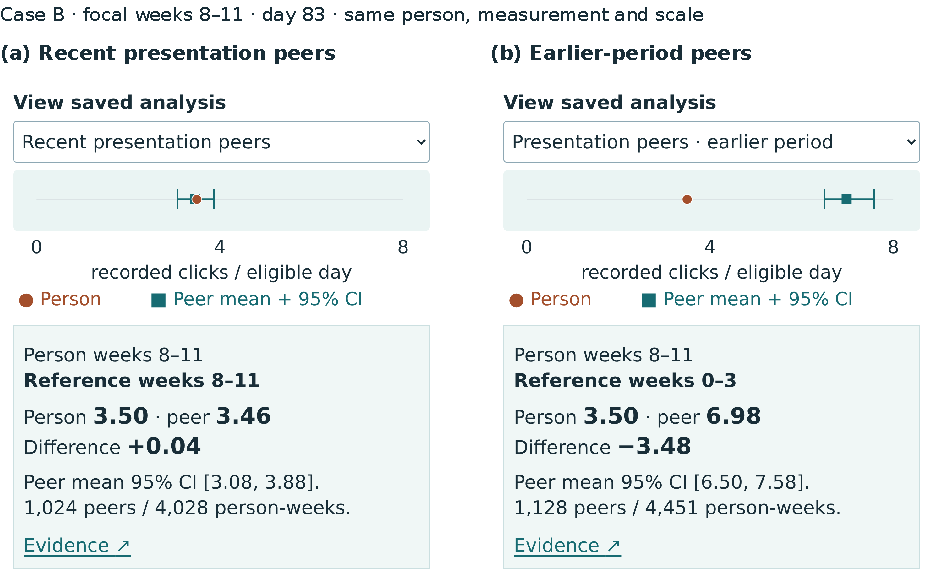
\includegraphics[width=\textwidth]{figures/reference_switch.pdf}
%DIFDELCMD < %%%
\DIFdelendFL \DIFaddbeginFL 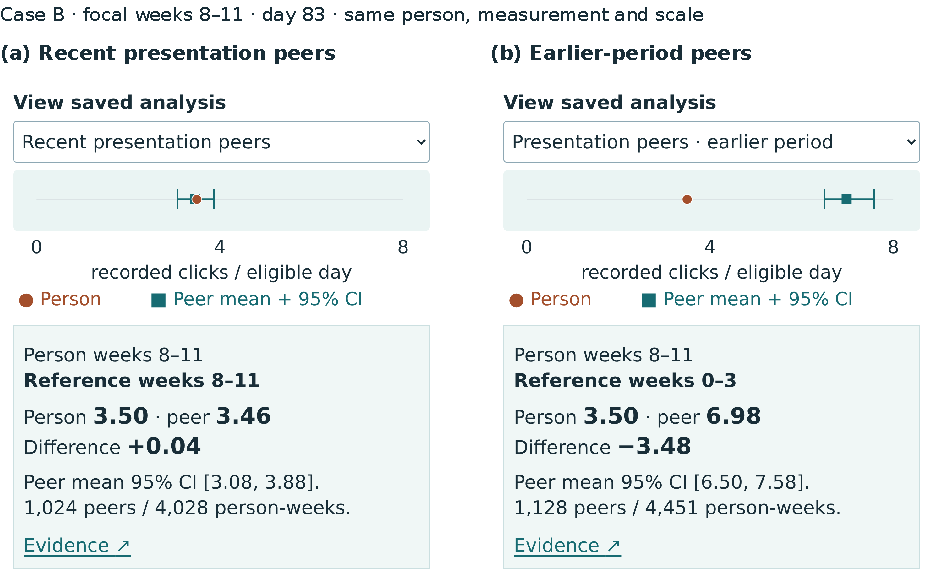
\includegraphics[width=0.9\textwidth]{figures/reference_switch.pdf}
\DIFaddendFL \caption{\DIFdelbeginFL \DIFdelFL{A saved reference-period change in condition A, case~05. Both comparisons were }\DIFdelendFL \DIFaddbeginFL \DIFaddFL{Saved }\DIFaddendFL model-selected \DIFdelbeginFL \DIFdelFL{. Browser excerpts show the selector reading validated records, not recomputing statistics}\DIFdelendFL \DIFaddbeginFL \DIFaddFL{comparisons in A05}\DIFaddendFL . The \DIFaddbeginFL \DIFaddFL{focal }\DIFaddendFL person, \DIFdelbeginFL \DIFdelFL{focal }\DIFdelendFL weeks \DIFdelbeginFL \DIFdelFL{~8-11}\DIFdelendFL \DIFaddbeginFL \DIFaddFL{8--11}\DIFaddendFL , units, and scale stay fixed\DIFdelbeginFL \DIFdelFL{and the }\DIFdelendFL \DIFaddbeginFL \DIFaddFL{; }\DIFaddendFL reference \DIFdelbeginFL \DIFdelFL{changes from }\DIFdelendFL weeks \DIFdelbeginFL \DIFdelFL{~8-11 }\DIFdelendFL \DIFaddbeginFL \DIFaddFL{change from 8--11 }\DIFaddendFL to \DIFdelbeginFL \DIFdelFL{weeks~0-3. Eligible membership differs }\DIFdelendFL \DIFaddbeginFL \DIFaddFL{0--3 }\DIFaddendFL (1,024 versus 1,128 \DIFdelbeginFL \DIFdelFL{people}\DIFdelendFL \DIFaddbeginFL \DIFaddFL{peers}\DIFaddendFL ). \DIFaddbeginFL \DIFaddFL{The selector reads saved results without recalculation. }\DIFaddendFL Whiskers are 95\% bootstrap intervals for peer means, not \DIFdelbeginFL \DIFdelFL{for }\DIFdelendFL contrasts. \DIFdelbeginFL \DIFdelFL{The later presentation layer supplies the layout. }\DIFdelendFL Earlier peers are not necessarily fairer or causally adjusted.}
\label{fig:reference}
\end{figure*}

\subsection{\DIFdelbegin \DIFdel{Recorded Cost}\DIFdelend \DIFaddbegin \DIFadd{Post Hoc Statistical and Data-Quality Checks}\DIFaddend }
\DIFdelbegin \DIFdel{Table~3 retains failures and repairs. Enumeration used more calls but far less episode time and no inference. C used more generations and equivalent repeated analyses than either control without higher completeness. This supports enumeration's operational economy within the registry.
}%DIFDELCMD < 

%DIFDELCMD < \begin{table*}[!t]
%DIFDELCMD < %%%
%DIFDELCMD < \caption{%
{%DIFAUXCMD
\DIFdelFL{Recorded comparison costs summed over 24 cases per condition. Episode time includes analytical and rendering work, shared model loading/profiling is separate. $^{a}$Exact/equivalent repeated requests use the frozen signatures; equivalent requests share feature, group and window meaning. Input/output token totals count repeated context, failures, and repairs.}}
%DIFAUXCMD
%DIFDELCMD < \label{tab:costs}
%DIFDELCMD < \centering\setlength{\tabcolsep}{3pt}
%DIFDELCMD < %%%
%DIF <  BEGIN GENERATED: costs
%DIF < % Generated from frozen reports; do not edit.
%DIFDELCMD < \begin{tabular}{lrrrrrr}
%DIFDELCMD < \hline
%DIFDELCMD < %%%
\DIFdelFL{Condition }%DIFDELCMD < & %%%
\DIFdelFL{Tools }%DIFDELCMD < & %%%
\DIFdelFL{Repeated$^{a}$ }%DIFDELCMD < & %%%
\DIFdelFL{Generations }%DIFDELCMD < & %%%
\DIFdelFL{Input / output tokens }%DIFDELCMD < & %%%
\DIFdelFL{Episode s }%DIFDELCMD < & %%%
\DIFdelFL{Median s }%DIFDELCMD < \\
%DIFDELCMD < \hline
%DIFDELCMD < %%%
\DIFdelFL{Enumeration }%DIFDELCMD < & %%%
\DIFdelFL{84 }%DIFDELCMD < & %%%
\DIFdelFL{0 / 0 }%DIFDELCMD < & %%%
\DIFdelFL{0 }%DIFDELCMD < & %%%
\DIFdelFL{0 / 0 }%DIFDELCMD < & %%%
\DIFdelFL{35.40 }%DIFDELCMD < & %%%
\DIFdelFL{1.18 }%DIFDELCMD < \\
%DIFDELCMD < %%%
\DIFdelFL{A: compact }%DIFDELCMD < & %%%
\DIFdelFL{76 }%DIFDELCMD < & %%%
\DIFdelFL{0 / 5 }%DIFDELCMD < & %%%
\DIFdelFL{52 }%DIFDELCMD < & %%%
\DIFdelFL{178, 794 / 10, 274 }%DIFDELCMD < & %%%
\DIFdelFL{484.64 }%DIFDELCMD < & %%%
\DIFdelFL{17.07 }%DIFDELCMD < \\
%DIFDELCMD < %%%
\DIFdelFL{B : derived metadata }%DIFDELCMD < & %%%
\DIFdelFL{79 }%DIFDELCMD < & %%%
\DIFdelFL{0 / 8 }%DIFDELCMD < & %%%
\DIFdelFL{53 }%DIFDELCMD < & %%%
\DIFdelFL{238,675 }\DIFdelendFL \DIFaddbeginFL \label{sec:sensitivity}
\DIFaddFL{To address statistical comparison, we applied two-sided exact McNemar tests to paired complete-visible outcomes, with Holm adjustment across all six condition pairs. The unit is the person, not the 96 method}\DIFaddendFL /\DIFdelbeginFL \DIFdelFL{10}\DIFdelendFL \DIFaddbeginFL \DIFaddFL{case slots. C--A and B--A each differ by $-25$ percentage points (adjusted $p=0.2813$); C--B differs by zero ($p=1$). Against enumeration}\DIFaddendFL , \DIFdelbeginFL \DIFdelFL{012 }%DIFDELCMD < & %%%
\DIFdelFL{504.21 }%DIFDELCMD < & %%%
\DIFdelFL{16.87 }%DIFDELCMD < \\
%DIFDELCMD < %%%
\DIFdelFL{C : explicit binding }%DIFDELCMD < & %%%
\DIFdelFL{82 }%DIFDELCMD < & %%%
\DIFdelFL{4 / 12 }%DIFDELCMD < & %%%
\DIFdelFL{63 }%DIFDELCMD < & %%%
\DIFdelFL{262, 031 }\DIFdelendFL \DIFaddbeginFL \DIFaddFL{A differs by $-12.5$ points ($p=0.5000$), and B and C each by $-37.5$ points ($p=0.0234$ each). Under the conditional B17--20 credit, B differs from enumeration by $-20.8$ points ($p=0.3125$ after the same six-test adjustment). These exploratory tests assume independent paired cases; shared course}\DIFaddendFL /\DIFdelbeginFL \DIFdelFL{10,695 }%DIFDELCMD < & %%%
\DIFdelFL{536.32 }%DIFDELCMD < & %%%
\DIFdelFL{21.19 }%DIFDELCMD < \\
%DIFDELCMD < \hline
%DIFDELCMD < \end{tabular}
%DIFDELCMD < %%%
%DIF <  END GENERATED: costs
%DIFDELCMD < \space %%%
%DIF <  Preserve the trailing space from the original table input.
%DIFDELCMD < \end{table*}
%DIFDELCMD < %%%
\DIFdelend \DIFaddbegin \DIFadd{reference pools and structural selection limit inferential interpretation. Non-rejection does not establish equivalence or held-out reliability.
}\DIFaddend 

\DIFdelbegin \DIFdel{Including setup/construction, 185 generations used 1, 719.02~s of model-process time (28.65~min), including loading/cleanup: 153.02~s construction and 1,566.00~s comparison. Shared comparison loading/profiling took 37.55}\DIFdelend \DIFaddbegin \DIFadd{Using preserved features with exact repeated source rows removed, we repeated the numerical comparisons for the same 24 people, profiles, and 81 peer exclusions. Of 52 required feature}\DIFaddend /\DIFdelbegin \DIFdel{1.65~s. Peak allocated}\DIFdelend \DIFaddbegin \DIFadd{reference records, all 29 supported click-rate peer contrasts and all 13 supported personal changes retained their signs. Median}\DIFaddend /\DIFdelbegin \DIFdel{reserved memory was 30.78}\DIFdelend \DIFaddbegin \DIFadd{maximum absolute peer-contrast shifts were 0.167}\DIFaddend /\DIFdelbegin \DIFdel{35.23~GiB; maximum input was 10}\DIFdelend \DIFaddbegin \DIFadd{0.324 clicks per eligible day; the maximum personal-change shift was 1.393. All 16 assessment records, support statuses, and eight cross-reference direction conclusions were unchanged. In Figure~\ref{fig:reference}, +0.043 and $-3.480$ become +0.088 and $-3.335$. This post hoc check does not identify unique click events or establish robustness of agent selections. Intervals were not recomputed; no agents were rerun and completeness scores were unchanged.
}

\DIFadd{Across 24 cases, enumeration took 35.40~s, compared with 484.64, 504.21, and 536.32~s for A, B}\DIFaddend , \DIFdelbegin \DIFdel{888 tokens. Process time, episode latency, and implementation wall time differ and do not establish billing time. Manuscript preparation ran no experimental inference}\DIFdelend \DIFaddbegin \DIFadd{and C}\DIFaddend . \DIFaddbegin \DIFadd{These descriptive episode totals include failed runs and repairs but exclude shared model loading; enumeration used no inference.
}\DIFaddend 

\section{\uppercase{Discussion and Limitations}}
\label{sec:discussion}
\DIFdelbegin %DIFDELCMD < \noindent %%%
\DIFdel{The study demonstrates a practical architecture for combining agent selection, deterministic analysis, and adaptive dashboard views. Its central methodological contribution is making the path from a question to its displayed answer inspectable. This allows developers to distinguish calculation errors, unsuitable selections, missing answers, and context added automatically by the software. Case~15 illustrates the value of this separation. The agent identifies insufficient personal observations but selects earlier peer comparisons for a question about recent activity. Preserving that output exposes a specific selection problem that automatic completion would conceal.
}%DIFDELCMD < 

%DIFDELCMD < \begin{figure*}[!t]
%DIFDELCMD < \centering
%DIFDELCMD < \includegraphics[width=\textwidth]{figures/failure.pdf}
%DIFDELCMD < %%%
%DIFDELCMD < \caption{%
{%DIFAUXCMD
\DIFdelFL{Inspecting an incomplete answer with correctly sourced values in case~15. The question concerns weeks~10--11 and asks separately about personal history and peers. (a) A selects peer comparisons for weeks~0--3 and retains a personal insufficiency answer. (b) Enumeration supplies both personal and recent peer insufficiency answers. Annotations outside the original excerpts identify the mismatch without inserting the missing answer. Evaluation uses the full original dashboards. Intervals describe peer means, and unavailable values remain distinct from zero.}}
%DIFAUXCMD
%DIFDELCMD < \label{fig:failure}
%DIFDELCMD < \end{figure*}
%DIFDELCMD < 

%DIFDELCMD < %%%
\DIFdelend \subsection{Lessons for Dashboard Design}
\DIFdelbegin \DIFdel{Compact Aachieved the highest frozen agent completeness. Baccepted more outputs, while C's explicit identifiers produced no gain in complete visible answers over B. These results show why successful construction and answer coverage should be assessed separately. B changes both metadata handling and catalogue availability, so its comparison with A evaluates that combined interface design. The traces identify concrete development priorities, including selecting the requested period, constructing valid requests, and covering every part of a question.
}%DIFDELCMD < 

%DIFDELCMD < %%%
\DIFdel{The attribution method also distinguishes model contributions from software assistance.
}\DIFdelend Automatically supplied context can complete an answer without \DIFdelbegin \DIFdel{having been selected by the model . Conversely, }\DIFdelend \DIFaddbegin \DIFadd{model selection, while }\DIFaddend B17--20 \DIFdelbegin \DIFdel{contain requested values in forms that the frozen evaluator does not credit. Recording both content and its origin supports a more informative assessment than counting panels or accepted outputs alone. Equivalent answer forms still require human adjudication.
Enumeration provides a reproducible operational baseline for the current registryand known task families. The shared backend makes its comparison with agents useful for assessing the cost and completeness of selection. Whether agents offer advantages for ambiguous questions , larger analysis libraries, or other domains remains a question for subsequent evaluation}\DIFdelend \DIFaddbegin \DIFadd{show that an evaluator can miss equivalent answer forms. Both content and origin therefore matter.
}

\DIFadd{For these structured questions and the small reference registry, the results establish no added agent value over enumeration. A possible role is translating less structured or ambiguous questions into analytical choices when enumerating a larger library is impractical. That role requires a separate comparison using ambiguous questions, clarification behavior, and matched budgets; it was not tested here}\DIFaddend .

\subsection{Adaptive Views and Operator Context}
\DIFdelbegin \DIFdel{The interface examples show how the same analytical foundation supports different questions. }\DIFdelend In Figure~\ref{fig:reference}, the person's rate \DIFdelbegin \DIFdel{remains }\DIFdelend \DIFaddbegin \DIFadd{stays }\DIFaddend 3.50 clicks per eligible day while recent and earlier peer means are 3.46 and 6.98\DIFdelbegin \DIFdel{. The corresponding differences are }\DIFdelend \DIFaddbegin \DIFadd{, giving differences }\DIFaddend +0.04 and $-3.48$ \DIFdelbegin \DIFdel{, calculated }\DIFdelend before rounding. \DIFdelbegin \DIFdel{Displaying the periods }\DIFdelend \DIFaddbegin \DIFadd{Periods }\DIFaddend and membership counts \DIFdelbegin \DIFdel{makes }\DIFdelend \DIFaddbegin \DIFadd{make }\DIFaddend the reference choice inspectable without \DIFdelbegin \DIFdel{suggesting that one group is inherently preferable or that the difference is causal }\DIFdelend \DIFaddbegin \DIFadd{implying a preferable or causal comparison}\DIFaddend .

\DIFdelbegin \DIFdel{Assessment views preserve the timing needed to interpret apparently conflicting records. In A17, weeks~8--11 contain 0.25 non-banked submissions per observed week and zero scheduled non-submissions. A day-55 snapshot nevertheless records no submission for the day-54 assessment. These summaries describe different periods, and later submissions do not rewrite earlier snapshots}\DIFdelend \DIFaddbegin \DIFadd{The graphical trajectories describe recorded activity, not knowledge acquisition. No dashboard intervention or learning-outcome study was conducted, so improvement in students' results or learning cannot be inferred}\DIFaddend . Grades and banking approval remain unavailable. \DIFdelbegin \DIFdel{The examples demonstrate implemented adaptation, while its effects }\DIFdelend \DIFaddbegin \DIFadd{Effects }\DIFaddend on operator understanding and usability \DIFaddbegin \DIFadd{also }\DIFaddend require direct evaluation.

\subsection{Scope and Further Validation}
The comparison covers 24 development people from two offerings\DIFdelbegin \DIFdel{. Its 96 outputs are paired method comparisons, not independent participants. Task }\DIFdelend \DIFaddbegin \DIFadd{, with known }\DIFaddend families and wording \DIFdelbegin \DIFdel{were known, }\DIFdelend and one checkpoint \DIFdelbegin \DIFdel{with greedy decodingdoes not establish performance across models, paraphrases, or deployments. Reserved peopleremain unevaluated, and earlier development provides no independent confirmation. The next validation step should resolve these judgments before fixing }\DIFdelend \DIFaddbegin \DIFadd{under greedy decoding. Additional independent test cases, preferably reserved people, have not been evaluated. Answer-equivalence judgments should be resolved before locking }\DIFaddend the system, evaluator, outcomes, and \DIFdelbegin \DIFdel{person-level }\DIFdelend sampling plan for reserved data. \DIFdelbegin \DIFdel{Any revised scoring should preserve the original results and be reported as a separate post hoc analysis. This progression builds on the implemented tool and its documented examples while keeping stronger reliability claims tied to independent evidence}\DIFdelend \DIFaddbegin \DIFadd{A user study should compare interpretation accuracy, completion time, and missing-value/reference errors against a fixed dashboard; no such outcomes are available. New analyses here reuse development cases and do not replace independent validation. Any adjudicated scores should be reported separately from the frozen results}\DIFaddend .
 OpenAI Codex \cite{openaiCodex} assisted with the programming environment, figure production and language editing.


\section{\uppercase{Conclusion}}
\label{sec:conclusion}
\noindent \DIFdelbegin \DIFdel{The implemented dashboards connect agent selections with deterministic calculations, traceable evidence, and reusable presentation templates. Personal timelines, peer comparisons, observation summaries, and assessment views support different questions through shared analyses. Operators can inspect supporting records and switch among saved comparisons while retaining their analytical context.
}%DIFDELCMD < 

%DIFDELCMD < %%%
\DIFdelend Across 24 development cases, explicit analytical identifiers did not improve frozen completeness, while enumeration remained complete and cheaper. \DIFdelbegin \DIFdel{The evaluation nevertheless provides concrete guidance for system development. }\DIFdelend Correctly calculated values can refer to the wrong period or leave a question partly unanswered, while automatically supplied context can complete an answer without model selection\DIFdelbegin \DIFdel{. Tracking these contributions separately makes both successful behavior and remaining selection problems visible.
}%DIFDELCMD < 

%DIFDELCMD < %%%
\DIFdel{The contribution combines a working tool, interface examples, and reproducible evaluation of answer completeness}\DIFdelend . 
Answer equivalence and measurement choices require review before validation on reserved data. Evaluation should examine operator understanding and usability. 


%\section{\uppercase{AI Assistance Disclosure}}
%\label{sec:disclosure}
%\noindent OpenAI Codex \cite{openaiCodex} assisted with the develop. The experimental model was Qwen2.5-14B-Instruct. Figures depict saved results or programmatic diagrams. The authors retain responsibility for the content.


\bibliographystyle{apalike}
\bibliography{references}
\end{document}
